\subsection{General static-kernel tomography on the actual source}
\label{sec:general-tomography-12}

The eleven-state experiment above identifies eight Walsh-diagonal
coefficients. A general real symmetric $8\times8$ kernel has 36
coefficients and requires a different design. Let the unnormalized Walsh
density be $\rho_q=\sum_x(-1)^{\operatorname{popcount}(q\mathbin{\&}x)}\rho_x$.
On literal source columns $X$ its energy matrix is
\begin{equation}
 K_B=-\tfrac18\sum_{q,r=0}^7B_{qr}X^*\rho_q\rho_rX,
 \qquad B=B^T\in\mathbb R^{8\times8}.
\end{equation}
First act with every density on the physical CAR parent, obtaining
$D_q=\rho_qX$, and then contract $M_{qr}=D_q^*D_r$.
Replacing this product by $(X^*\rho_qX)(X^*\rho_rX)$ drops physical
image directions. A normalized original phase source misses six units
in the $\rho_4^2$ diagonal by that shortcut; edge 7 misses eight.
\samref{REF12_ONE}

For real columns, the complete design has rows
$C_{(i,j),(q,r)}=(2-\delta_{qr})(M_{qr})_{ij}$,
$i\le j$, $q\le r$. Its phase 9 rank is 18 with nullity 18;
the source11 rank is 21 with nullity 15. Exact nonzero minors and complete
exact null products establish both bounds. In particular the symmetric
perturbation $B_{15}=1$, $B_{04}=-1/6$ is invisible on source11.
An additional actual source600 direction $(0,0,5,2)$, paired with
originalphase0, has raw response 24 before the $-1/8$ factor. This is a
reachable repair of that null, not a symmetry-null test.

Eighteen literal physical source vectors supply two complete designs.
They comprise phase 9, the ground-$u$ and $t1,d1$ pair directions, and
the seven Fourier-pair directions
\begin{equation}
\begin{gathered}
(0,0,1,2),(0,0,2,1),(0,0,2,4),(0,0,4,1),\\
(0,0,4,2),(0,0,4,4),(0,0,5,2).
\end{gathered}
\end{equation}
Fixed integer $18\times8$ and Gaussian-integer $18\times6$ transforms
give real-eight and complex-six source spans. The report retained with
this edition prints all 18 sparse exterior columns and both transforms;
the exact design/inverse arrays accompany it. Physical CAR signs use
ascending Fourier modes within flavors ordered proton-up, proton-down,
neutron-up, neutron-down. No source coefficient is chosen by a desired
binding value.

For the real span, all 36 upper-triangular energy entries form an
invertible design. For the complex span, use the six diagonal real
entries followed by real and imaginary parts of its 15 upper entries.
Both exact inverses obey $CC^{-1}=I$, entry by entry, and separate native
certified solves enclose every rational inverse entry. For an exact
specification independent of decimal printout,
\begin{equation}
 (C^{-1})_{ij}=(-1)^{i+j}
                  \det C_{\widehat j,\widehat i}/\det C.
\end{equation}
Seven real directions have at most 28 symmetric entries, and five complex
directions at most 25 Hermitian real entries. Eight and six are therefore
minimal \emph{span dimensions}. The real design needs 64 scalar readings
under polarization; the complex one needs 66 and calibrated relative
phases. This does not prove a minimum number of physical preparations.

\begin{figure}[htbp]\centering
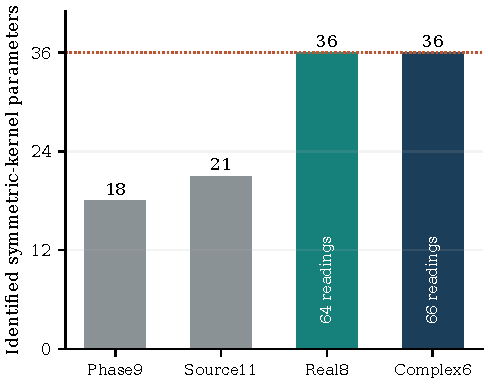
\includegraphics[width=\columnwidth]{refinement_20261112/figures/tomography_rank.pdf}
\caption{General symmetric-kernel identification. The phase 9 and
source11 ranks leave genuine invisible directions. The two repaired
designs identify all 36 parameters on minimal real or complex source
spans; their reading counts and phase requirements differ.}
\label{fig:tomography-rank-12}
\end{figure}

Suppose normalized scalar energy readings have absolute error at most
$\varepsilon$, with actual source Gram $G$, kinetic subtraction and
absolute common zero separately known. Diagonal unnormalized error is
at most $G_{ii}\varepsilon$, and each polarized off-diagonal real or
imaginary error at most $(G_{ii}+G_{jj})\varepsilon/2$.
Let $w$ be these weights and $\beta=|C^{-1}|w$. Since the reconstructed
coefficient vector is $b=-8C^{-1}y$,
\begin{equation}
 \|\delta B\|\le8\max_q\sum_r
             \beta_{\min(q,r),\max(q,r)}\varepsilon.
\end{equation}
Exact rational comparisons give the outward sufficient constants
\begin{equation}
 \|\delta B\|\le
 \begin{cases}1325.485758855\,\varepsilon,&\text{real eight},\\
               2253.867579928\,\varepsilon,&\text{complex six}.
 \end{cases}
\label{eq:tomography-error-12}
\end{equation}
These general-kernel constants do not replace the smaller diagonal-family
constant in \eqref{eq:kernel-error-new}. Source preparation, metric,
kinetic and zero-reference errors remain separate payments. Fixed-number
energy differences alone cannot determine the absolute uniform mode.

\subsection{Branch-aware robustness and the dressed density recipient}
\label{sec:robustness-12}

The original conservative $20\delta$ proper-fragment payment can be
sharpened on a declared interval. Four-flavor Pauli occupation gives
$\sum_x\rho_x^2\le16\lfloor n/4\rfloor+(n\bmod4)^2$ for $n$ particles,
also across all cell allocations. Proper $5+1$ has cap 18, while $4+2$
has cap 20 but starts $20/3$ higher in its complete lower. The other
proper size types remain higher. Consequently
\begin{align}
 L_{\rm new}&\ge L_{\rm old}-18\delta,\\
 m_{{\rm old\ target},{\rm new}}
 &\ge\frac{11191}{20250}-\frac{23294}{675}\delta.
\end{align}
The interval is $0\le\delta\le10/3$. The sufficient old-target tolerance is $\delta<11191/698820$.
At $\delta=10/3+1/100$ the $4+2$ envelope falls below the claimed
$5+1$ envelope by $1/50$; the interval restriction is substantive.

For the improved cloud-dressed target \eqref{eq:one-hop-polar-12}, a new
full density-square contraction is needed. Write
$D_2=\sum_{R,x}\rho_{R,x}^2$ and
$W_\lambda=J_\lambda^*KD_2KJ_\lambda$. Parity gives
\begin{equation}
 J_{\lambda,\alpha}^*D_2J_{\lambda,\alpha}
 =C_\lambda(s_\lambda I+\alpha_\lambda^2W_\lambda)C_\lambda,
 \quad C_\lambda=(I+\alpha_\lambda^2V_\lambda)^{-1/2},
\end{equation}
where $(s_{42},s_{33},s_{321})=(20,18,14)$.
Signed one-hop image products retain the actual coherent overlaps and
cell escapes. With their exact exponential ceilings, the sector density
uppers are $19.92490702818282\ldots$, $17.93969844791798\ldots$,
$13.94407489806138\ldots$. At the unchanged source weights their average is
\begin{equation}
 \overline S_\alpha=16.44780324393715\ldots.
\end{equation}
This differs from the bare target's $11144/675$; copying the old observable
to the dressed state would miss terms.

For the explicit common instantaneous full-Hamiltonian perturbation
$-\sum_R\rho_R^T\Delta B\rho_R$, $\|\Delta B\|\le\delta$, let the locked sufficient margin be
\begin{equation}
 M_\alpha=\frac{2139952734887423053027468631}
                  {1335165038749772953286830250}.
\end{equation}
Then
\begin{equation}
 m_{\alpha,\rm new}\ge
 M_\alpha-(18+\overline S_\alpha)\delta,\qquad0\le\delta\le10/3.
\end{equation}
The sufficient tolerance is $\delta<.0465272835531455\ldots$.
Combining with \eqref{eq:tomography-error-12}, before additional errors,
gives $\varepsilon<.0000351020622004667\ldots$ for real eight and
$\varepsilon<.0000206433084035217\ldots$ for complex six.
\samref{REF12_ONE}

A different receiver with the same calibrated static kernel can change
field clouds, poles and hopping response. If its transported trial has
additional energy-form error $\eta$, the valid margin is
$M_\alpha-(18+\overline S_\alpha)\delta-\eta$.
The explicit instantaneous perturbation has $\eta=0$; static calibration
alone cannot impose this on a changed field inertia or vertex law.

\subsection{A signed uniform mode is not a canceling rest reference}
\label{sec:uniform-mode-12}

For $B_{\rm new}=35G+\Delta\mathbf1\mathbf1^T/8$, the interaction shifts
by $-\Delta\sum_RN_R^2/8$. At $-1/2\le\Delta\le1/2$, all-cell fragment
slacks keep $5+1$ lowest. The original target has one-cell square 36 and
that split has square 26, so
\begin{equation}
 m_{{\rm old},{\rm new}}\ge11191/20250+5\Delta/4.
\end{equation}
Positivity is sufficient for $\Delta>-22382/50625$ within the stated
interval. An affine constituent rest baseline cancels at fixed inventory;
this quadratic occupancy interaction does not.

The one-hop trial has a small cell-escape probability. In sector $\lambda$,
$p_{{\rm cell},\lambda}=36t_c^2\alpha_\lambda^2\langle C_\lambda^2\rangle$,
and its actual square is $36-10p_{{\rm cell},\lambda}$.
The weighted probability is at most $1.65456182334269\,10^{-8}$.
Thus the positive-$\Delta$ margin slope is at least
$(5/4)(1-1.65456182334269\,10^{-8})$; the safe negative-$\Delta$ slope
remains $5/4$. Even this tiny physical cell term must accompany a claimed
exact response coefficient.
